\documentclass[oneside]{book}
% Add the packages
\usepackage{algorithm}
\usepackage{algpseudocode}
\usepackage{listings}
\usepackage{graphicx}
\usepackage{hyperref}
\usepackage{comment}
\hypersetup{%
    pdfborder = {0 0 0}
}

\usepackage[utf8]{inputenc}
\usepackage[T3,T1]{fontenc}
\usepackage[english]{babel}
\usepackage[noenc]{tipa}
\usepackage{tipx}
\usepackage{amssymb,amsfonts,textcomp}
\usepackage{array}
\usepackage{longtable}
\usepackage[margin=2.4cm,a4paper]{geometry}
\usepackage[T1]{fontenc}
\usepackage{supertabular}
\usepackage{hhline}
\makeatletter
\newcommand\arraybslash{\let\\\@arraycr}
\makeatother
\setlength\tabcolsep{1mm}
\renewcommand\arraystretch{1.3}

\begin{document}


\begin{titlepage}
	\centering
	
\includegraphics[width=0.15\textwidth]{logo-uva}\par\vspace{2.5mm}
	{\scshape\LARGE University of Amsterdam \par}
	\vspace{2mm}
	{\scshape\Large Master Thesis Project\par}
	\vspace{1.5cm}
	{\Huge\bfseries Forgery: Synthesizing Database Transactions\par}
	\vspace{1cm}
	{\Large\itshape Guy - Sean Rombaut\par}
	\vfill
	Supervised by:\par
	Dr.~Tijs van der Storm\par
	Jouke Stoel\par
	\vspace{1cm}
	Organizations:\par
		 Internationale Nederlanden Groep (ING) \hfill  
\includegraphics[width=0.15\textwidth]{ING}\par
	 Centrum Wiskunde \& Informatica (CWI)  \hfill  
\includegraphics[width=0.15\textwidth]{CWIlogo}

	\vfill

% Bottom of the page
	{\large \today\par}
\end{titlepage}

\tableofcontents
\newpage

\chapter{Abstract}
The popularity of modeling languages is increasing. This is mostly due to the fact that using modeling languages is an efficient way to end up with a high quality system \cite[p. ~6]{abstractions}. By providing immediate feedback to users they allow early detection of design errors \cite{lightning}. Nonetheless these models are far from being a real implemented product. Manual implementation is required which makes it more prone to mistakes. Our motivation for this research was to find a solution in this matter.\\

We decided to focus our research on the field of automatic database generation rather than whole programs as we found it very interesting. Considering the human factor, it is not possible to develop a fault-free software in practice \cite{reliability}. When those issues occur the data itself may also be effected and this makes it more difficult to repair. Data errors can harm the reputation of an organization, diminish financial gains and create uncertainty in an organization.\\

\textit{Forgery} is a tool for generating database schemes and synthesize transactions based on a predefined model. \textit{Forgery} uses \textit{Alloy} as a specification language for describing models and validating them. An \textit{Alloy} model is a collection of constraints and relations that describes a set of structures. Using pre- and postconditions it defines the operations that are allowed in the system. \textit{Forgery} converts them into database tables, procedures and structural constraints.

\begin{comment}
\textit{Fors} is a specific domain language (DSL) for modelling and specifying financial products based on pre- and post-conditions. It uses \textit{Alloy} to check the correctness of the model. \textit{Fors} was created to minimize the communications gap between technical and non-technical teams. However, it cannot guarantee the correctness of the implementation of the real product. Our research attempts to deal with the realization issue. We come into a solution from the data prospective. 


systems. We present Alchemy, which compiles Alloy specifi-
cations into implementations that execute against persistent
databases. Alchemy translates a subset of Alloy predicates
into imperative update operations, and it converts facts into
database integrity constraints that it maintains automati-
cally in the face of these imperative actions.
In addition to presenting the semantics and an algorithm
for this compilation, we present the tool and outline its
application to a non-trivial specification. We also discuss
lessons learned about the relationship between Alloy speci-
fications and imperative implementations
Synthesizing database transaction from a DSL for financial products
\end{comment}


\newpage

\chapter{Preface}

This research was done for the Dutch bank ING. The original project aimed to find a solution regarding the communication issues between technical and non-technical teams inside the organization. For example, specifications ambiguity or misunderstandings between the teams. The project was initially called \textit{Fors} and later on was renamed to \textit{Rebel}. \textit{Rebel} is a domain specific language (DSL) that parses business software specifications into algebraic-based language which is called \textit{Alloy}. With \textit{Alloy} it is possible to validate those specifications and create a model that the technical team can implement.\\

\textit{Forgery} aims to find a solution regarding faults in the process of the realization of a model. \textit{Forgery} continues the process of \textit{Fors} to support the realization. Together with \textit{Fors} we may achieve two things: better specifications and better realization.\\

\newpage

\chapter{Background}
This chapter discusses the background of developing \textit{Forgery}, the previous work that has been done and the motivation for it. It also contains the research question along with a description of the remaining chapters of this thesis.

\section{Motivation}

The success of implementing software projects is directly affected by the quality of its specifications \cite[p.~12]{requirements}. The specifications are typically defined based on two conceptual views: business and technical and are usually defined by different teams or people with various backgrounds. The gap between those two different perspectives may lead to costly misunderstandings \cite[p.~1]{fors}. Changing specifications after implementation of software often takes much more time and is also more expensive \cite{defectstopten}.\\

Today several tools exist for modeling and verifying software specifications. Examples are $Alloy$ and $Z-notation$. These tools allow software engineers to create prototypes of their ideas and identify errors, before realization. \\

However, sometimes such modeling tools seems to be too complicated. Even though the mathematical notations of these tools are unambiguous, the use of set theories, logic and algebra requires special expertise \cite[p.~10]{fors}. In addition, these tools are useful especially for prototyping general models and less effective when it comes to specific domains. We focus on such a specific domain (financial systems). \\

Because of the above-mentioned, we aimed at creating a new tool that would be better suited for prototyping financial systems and could be used by both the business and the development teams. We have developed our own Domain Specific Language (DSL) and called it $Fors$ which derived from: Separating Configuration From Formal Specification \cite{fors}. The concept of a DSL is very simple: Instead of aiming to solve any kind of computing problem, DSLs aim to solve specific class of problems. \cite{dsl}. In our case the DSL aims to solve problems of financial systems.  \\

$Fors$ expresses the operations of a system in a language whose vocabulary, syntax and semantics are formally defined in an easy and natural way. This way, $Fors$ is comprehensible for both business and development teams. In addition, $Fors$ is able to check the correctness of a software model. $Fors$ parse formal specifications into $Alloy$ syntax: algebraic logic formulas based on the notion of relations (We will elaborate on this more later in this thesis). Using an $Alloy$ based engine we are able to solve such formulas and find ambiguities in a model. \\

$Fors$ minimizes the gap between the business and the technical views by creating a common language and the ability to identify contradictions or faults in a specific model. However, there is still a main issue that remains: Programmers will have to implement the real product by hand (according to the specifications). Hence, it is not guaranteed that the final results would be exactly the same as defined in the specifications. When considering human factor also this system  is prone to error. \\

Therefore, our motivation was to find out whether we would be able to create a tool for automatic system generation. We decided to scope our research on the data-side as we found it highly interesting. As mentioned previously, data errors can harm the reputation of an organization, diminish financial gains and create uncertainty  in an organization. Synthesizing the data may avoid such events.\\

Data is usually stored in a record-keeping system called a database. A database therefore is a repository for a collection of data files on which users may perform a variety of operations (e.g. adding, modifying or reading files)  \cite[p.~11]{introtodb}.\\

The scope of database is often described as having the following three aspects:
\begin{itemize}
  \item Data Structure - the structure is a representation of the arrangement, relationships, and contents of data \cite{datastruct}. The structure is described diagrammatically by the data schema.  
  \item Data Manipulation - the available operations that can be applied on the data. Mainly $CRUD$ (Create, Read, Update and Delete) operations.
  \item Data Integrity - refers to the accuracy and consistency (validity) of data over its lifecycle.
\end{itemize}

Using a database has numerous benefits that lay mostly in the fact that data control is centralized. First, redundancy can be reduced. In contrast to private files, by using a relational database it is possible to merge related or overlapping information. Second, by linking multiple rows and use of transactions we can avoid inconsistency (corollary of the previous point). Also, security (permissions) and standards (e.g. representation of the data) can be enforced. And last, sharing data between multiple workstations is easy \cite[p.~16]{introtodb}.\\

Since \textit{Fors} uses \textit{Alloy}; and \textit{Alloy} is based on relations, we researched if it is possible to make a link between \textit{Alloy} and relational databases; and then we may automatically generate a matching database.\\

A relational database consists of three main principles:
\begin{itemize}
	\item Tables are the logical structure (but physically they can be stored in multiple way - binary trees, hashing etc). 
	\item The information principle - the entire content of the database is represented in one and only one way.
	\item The operators available to the user derive from old state to a new one.
\end{itemize}

The reason that such a system called "relational" is because basically a relation is a mathematical term for a table and it doesn't only refer to entities and relationships \cite[p.~26]{introtodb}. A relational system is based on the relational model of data.\\

\textbf{Example -} Simple student grades system:

\begin{center}
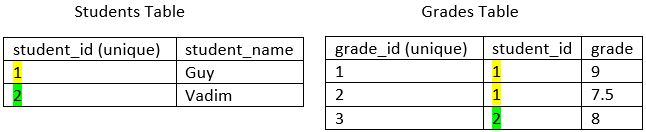
\includegraphics[scale=0.9]{table1}
\end{center}

Students table is storing students data (name), and grades table is used for storing the student grades. In order to make a link between a student and a grade we use a unique id. The user can use multiple operations to manipulate the data. Each operation (e.g. delete) will generate a new table; that means changing from "old" state to a "new" one. For example, by deleting a grade row, the relation will be replaced by a new one (excluding the deleted row). Similarly, inserting or updating operations.\\

Now we return back to relations. We have already mentioned the term "relation" multiple times. Before we can fully define a relation we have to introduce another term called $tuple$ due to the fact that tuples are a necessary stepping-stone to understand what a relation is.  Given a collection of types (e.g. number, date, address etc) $Ti(i=1,2,3...,n)$, a tuple value on those types - $t$, say - is a set of ordered triples of the form $<Ai,Ti,vi>$, where $Ai$ is an attribute name, $Ti$ is a type name and $vi$ is a value of type $Ti$. The value $n$ is the arity of $t$ (unary, binary etc) \cite[p.~142]{introtodb}.\\
$t(n)=<<A1, T1, v1>, <A2, T2, v2>..., <An, Tn, n>>$\\
Few notes regarding tuples:
\begin{itemize}
	\item The heading of $t$ is the set of attributes.
	\item The type of $t$ is determined by the types of its heading.
	\item Each tuple contains exactly one value for each of its attributes.
	\item Every subset of a tuple is a tuple.
	\item There are no duplicate tuples.
\end{itemize}
\textbf{Example -} Tuple: $Students = {<Student, Guy>, <Student, Vadim>}$\\
And now, here is the precise definition of a relation \cite[p.~146]{introtodb}. A relation $r$ consists of heading and a body, where:
\begin{itemize}
	\item The heading of $r$ is a tuple heading as defined before.
	\item The body of $r$ is a set of tuples with identical headings.
\end{itemize}
\textbf{Example -} Relation: 
$Grades = \{<<Student, Guy>, <Grade, 9>>,\\
<<Student, Guy>, <Grade, 7.5>>,\\
<<Student, Vadim>, <Grade, 8>>\}$\\

And lastly, the relations theory provides a set of operations for relations. For example, subset of $\subset$, superset of $\supset$, equals $=$ and others. Those will also be discussed in the next chapters.\\

As said, \textit{Alloy} is also based on the notion of relations and it use them as its main structure. Therefore, the data model of \textit{Alloy's} can be translated directly into persistent database schema. Obviously, \textit{Alloy} is much more than a data structure, it provides functions and more. We will discuss more about \textit{Alloy} in the next chapter.\\

We decided to use SQL (Structured Query Language) for the automation of database generating. SQL is a declarative language designed for constructing relational databases and managing the data that is held in it.\\

\begin{comment}
The results of software defects are expensive. Except for finding and fixing those defects, it may have huge effect on the data. Personally, I have experienced such a thing in my previous job: A bug in the calculation of a promotion was leaded to storing wrong amounts in the database. The company lost that money as the bills were already sent to the customers and it was irrevertible. Our research will attempt to find a solution to avoid such mistakes \cite{minimizingdefects}.
In this paper, we will not discuss about \textit{Fors} nor \textit{Alloy} in details. We assume that the reader has a general background about the idea of those two projects. For your convenience we included a quick reference in the appendix.\\
\end{comment}

\section{Problem Analysis}

Generating a database system automatically using only \textit{Alloy} specifications seems to be hard. We will cover the reasons in this section.

\subsection{Data Structure}

Although \textit{Alloy} relations and database tables are both based on the theory of relations, their structural representation is different.\\

\begin{itemize}
	\item Database tables are two-dimensional, while relations can have multiple dimensions.
	\item Database tables are ordered (top-bottom and left-right), while relations not.
	\item Database tables can contain empty data (null) and duplicates, while relations/tuples not.
	\item Each relation usually involve a type name. When it comes to database tables, types are typically omitted.
\end{itemize}

In addition, database systems make use of $Keys$ which are a vital part of the table structure. For example, $Primary$, $Foreign$ and $Unique$ Keys. \textit{Alloy} deals with it partially or not at all.\\ 

In order to be able to generate tables that can represent the corresponding \textit{Alloy} relations, we need to agree on certain rules of interpreting these relations (e.g. row or columns orderings are irrelevant) \cite[p.~151]{introtodb}.

\subsection{Data Operations}

Alloy uses $predicates$ as operations system. It allows users to create customized actions for modifying the data in the system using preconditions, postconditons and algebraic formulas (We will discuss about it in the next chapter). In database systems the core operations involve insert, update or delete. We need to bridge between algebraic notation and a SQL query notation.\\

Moreover, as mentioned before, in database systems the operators available to the user derive from old state to a new one. In \textit{Alloy} this is not necessarily the case. We need to enforce the specifications to follow that way.\\

And lastly, we have to assure that the new state is valid (according to the specified conditions of the formula). For example, \textit{Alloy} allows setting multiple operations inside single predicate. In database systems, each operation is discrete and it may occur that one operation succeeded and the following one didn't. In this case, the new state is invalid. To solve this for example, we can use transactions.\\

We will discuss about the solutions and the related work in the next few chapters.

\begin{comment}
MOVE TO RELATED WORK
Generating an entire system automatically based only on specifications seems to be extremely hard. The specifications in \textit{Alloy} describes a core model but a software is much more than that; Sometimes it has to deal with graphics and other complicated processes that cannot be fully specified or even aimed to be changed. Therefore, instead, we chose to focus on the validity of the data as this is the most important in most cases. And also, while the first approach may be impossible to achieve, the second would be much more reasonable. Generating a database system with constraints may guarantee that at least the data would be valid.\\

We based our research on a similar one which is known as \textit{Alchemy} \cite{alchemy} and have decided to replicate it. \textit{Alchemy} translates a subset of \textit{Alloy} specifications into a database scheme and APIs for performing data operations with some constraints.\\

During our research we have discovered that \textit{Alchemy} has some significant issues. First, \textit{Alchemy} does not have any systemic validation mechanism. It is impossible to check or verify how \textit{Alchemy} performs in different situations and there is a possibility that the results are different than those we are trying to achieve. Secondly, \textit{Alloy} offers $Assertions$ \cite[p. ~119]{abstractions} as a powerful testing tool. $Assertion$ is a constraint that is intended to follow from the invariants of the model. The built-in Analyzer can check the predicates using those assertions and if one of them violates the invariants, a counterexample is created. Such counterexamples may be very useful to validate our system and particularly the predicates. However, $Assertions$ cannot be used in \textit{Alchemy} because it uses a database auto-repair mechanism. This mechanism tries to find contradictions in the update and fix them. However, such events may occur only when the model or the invariants were specified incorrectly. In other words, it allows to create an invalid model \cite[p.~4]{alchemy}. In that case, if $Assertions$ were used, the built-in Analyzer would find it as a violation in the model.\\

In addition, $Alchemy$ uses an external API that check the constrains. Applying constraints within the database itself would be much more secured and better in terms of data integrity. It can ensure that data would not be modified in an unauthorized or improper way \cite[p.~2]{security}. Moreover, the generated scheme structure is far than being a natural database as it uses a single table for all the data. Although it doesn't seem to be an issue, we have to remember what $Fors$ was trying to achieve: clarity for both developers and business teams.\\

\textit{Forgery} tries to overcome with these problems using a different approach. \textit{Forgery} generates a pure SQL query that is used to construct full-scale database. $Signatures$ are converted into relational tables with $Foreign$ keys based on the specified relations and $Unique$ keys based on $cardinalities$. We will discuss it into details in \ref{sec:schemegen}.\\ 

$Facts$ are converted into database procedures that are used for the data validation, and $Predicates$ into inserting, updating or deleting procedures. All operations occurred transactionally so a failure of one of the operation will lead to a revert action. We will discuss it into details in \ref{sec:predicatesgen}.\\

\textit{Forgery} perform a reverse engineering on the  \textit{Alloy} solved models and use back-traces to validate and test the generated database system by emulating the operations and comparing the results to those who exists in Alloy (the $atoms$). We will discuss it into details in \ref{sec:validation}.\\ 
\end{comment}

\section{Research Question}

This paper researches the implementation problem and tries to answer the following question:\\

\textit{\textbf{How to bridge between Alloy-based specifications and realization?}}\\

To answer this question, the following sub-questions have been formulated:
\begin{itemize}
  \item How can we meet Alloy specifications?
  \item What are the limitations on Alloy specifications?
  \item How to validate that Forgery works?
\end{itemize}

\newpage

\chapter{Alloy}

Alloy is a declarative specification language for describing models with structural constraints and behavior used for modeling software systems. In addition, it includes a tool called Alloy Analyzer for visualizing models, exploring and checking the properties of them.\\

In this chapter we concentrate on the language part of Alloy, and we will provide few examples as demonstration. We will not cover the whole language but mostly what is required in order to understand this mass.\\

\section{Data Structure}

Alloy data model is based on $atoms$, $signatures$ and $fields$. Atom is the most basic element in Alloy which belong to a specific type. \textbf{sig}nature is a set of atoms, which also define the data type. A field describes relation between different types of signatures. It is a set of tuples which consists different types of data. Such a relation can be unary or binary (using →).\\

The following example describes a price list (tariff) of products in shop. 

\begin{lstlisting}
sig Price {}
sig Product {}
sig Shop {
	  tariff: Price -> Product
}
\end{lstlisting}

The signatures are $price$, $product$ and $shop$. The tariff describes the relation between each product and price within the shop. Running the Alloy Analyzer will generate all possible examples that follows the model. For example we may have two shops, with two different products that has the same price. In that case, we have two atoms of type shop, two atoms of type product, and single atom of type price.

\begin{center}
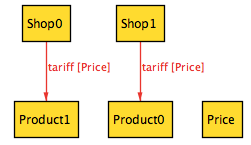
\includegraphics[scale=0.6]{shops1}
\end{center}

\subsection{Cardinalities}

Cardinality refers to the amount of elements in a set. Alloy allows us to set cardinality constraints on the data model. Alloy supports $lone$ (size is at most 1), $one$ (size is only 1), $some$ (size is at least 1), $no$ (size is 0). For example, let's assume that we want only one shop in our model:

\begin{lstlisting}
sig Price {}
sig Product {}
one sig Shop {
	  tariff: Price -> Product
}
\end{lstlisting}

Alloy Analyzer will now only generate examples with exactly one shop. 

\begin{center}
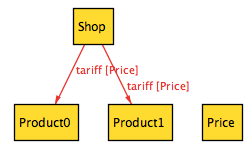
\includegraphics[scale=0.6]{shop2}
\end{center}

\section{Data Operations}
Alloy allows to define \textbf{pred}icates as an operations that act on that system. A predicate may convert a certain state of the data system into a new one, based on the rules it defines. The predicates accept signatures as an input, and the operations themselves defined using algebraic formulas. We may use semantics such as + (union), \& (intersection), in (subset), → (tupling), and . (join).\\

The following example describes a predicate that allows adding a new tariff (of product $pro$ with a price of $pri$ to the shop). The shop $s$ describes the old state while $s'$ describes the new state of the system.

\begin{lstlisting}
sig Price {}
sig Product {}
one sig Shop {
	  tariff: Price -> Product
}

pred AddTariff(s, s' : Shop, pro: Product, pri: Price) {
	  s'.tariff = s.tariff + (pri -> pro)
}
\end{lstlisting}

\begin{center}
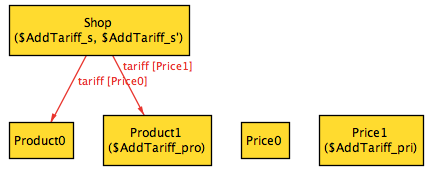
\includegraphics[scale=0.6]{shop3}
\end{center}

The shop had the product '0' with price '0' and after we added a product '1' with a price of '1'.

\section{Data Invariants}

Alloy allows to create system invariants using \textbf{fact}s. Those properties are meant to hold of all models constructed by Alloy. Any configuration that is an instance of the specification has to satisfy all the facts. In the previous example we could have products that doesn't belong to any shop ($Product0$).

\begin{center}
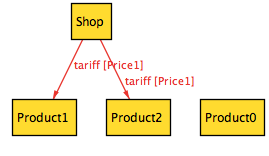
\includegraphics[scale=0.6]{shop4}
\end{center}

Using facts, we can assure, for example, that each product must belong to a shop.

\begin{lstlisting}
sig Price {}
sig Product {}
one sig Shop {
	  tariff: Price -> Product
}

pred AddTariff(s, s' : Shop, pro: Product, pri: Price) {
	  s'.tariff = s.tariff + (pri -> pro)
}

fact ProductMustHaveShop {
	all pro: Product | pro in Shop.tariff[Price]
}
\end{lstlisting}

\begin{center}
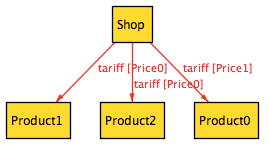
\includegraphics[scale=0.6]{shop5}
\end{center}

\section{Assertions}
Assertions are constraints that were intended to follow from facts of the model. \textbf{Assert}ions are used for checking that the desirable invariants exist using Alloy Analyzer. Alloy Analyzer tries to find counter examples that does not follow those constraints.\\

Let's assume that we want that each shop will have maximum one tariff, and such invariant was forgotten.

\begin{lstlisting}
sig Price {}
sig Product {}
one sig Shop {
	  tariff: Price -> Product
}

pred AddTariff(s, s' : Shop, pro: Product, pri: Price) {
	  s'.tariff = s.tariff + (pri -> pro)
}

fact ProductMustHaveShop {
	all pro: Product | pro in Shop.tariff[Price]
}

assert LoneTariff {
	all s: Shop | lone s.tariff
}
\end{lstlisting}

By running a check for the assertion \textit{LoneTariff}, Alloy Analyzer will alert that it found a counter example:

\begin{center}
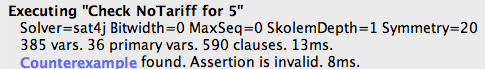
\includegraphics[scale=0.6]{counterexample}
\end{center}

By clicking on the counterexample, Alloy Analyzer will present the all counter-models. The following counterexample shows that there are more than one tariff, which is in conflict with the mentioned constrained. 

\begin{center}
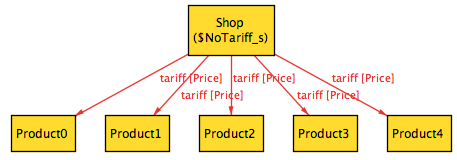
\includegraphics[scale=0.6]{counterexample1}
\end{center}

This way, we able to check our model, and make it more robust by minimizing mistakes.

\newpage

\chapter{Forgery Overview}
In this chapter we will briefly give an overview on the solution that we offer. It might give a general idea for those who are not interested in investing time reading it into details.

\section{Key Ingredients}

As introduced in the background Alloy specification consists of four main parts: Signatures (and their Cardinalities), Predicates, Facts and Assertions. Together they hint about how the model should be implemented. Using few examples we will demonstrate the conversion from Alloy specifications to implemented database.\\

The following example specifies a homework submission and grading system. 

\begin{lstlisting}
sig Submission { } 
sig Grade { }
sig Student { }
sig Course {
	roster: Student,
	work: roster -> Submission,
	gradebook: work -> Grade
}
\end{lstlisting}

For those specifications Alloy will generate multiple models. Arbitrarily we chose the following one:\\

\begin{center}
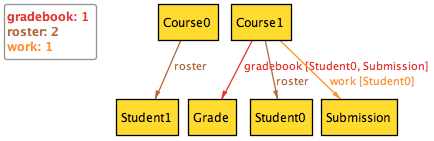
\includegraphics[scale=0.6]{overview1}
\end{center}

The system contains two courses, two student which are enrolled to each of those courses. Also, Student0 which is enrolled to Course1 submitted his work and got a grade for it.\\

First We need to generate a database schema for storing the data. As can be seen, Alloy Signatures can be translated directly into persistent database schemas. In Forgery, for each Signature we create a table, and for each field we create a junction tables that points to the relevant signature tables. Each Signature table stores its atoms. The relations set by ids which are the primary keys.\\

For example, the $student$ table is created by the following SQL code:

\begin{lstlisting}
CREATE TABLE `student`(
        `id` INT(6) UNSIGNED NOT NULL AUTO_INCREMENT PRIMARY KEY,
        `value` VARCHAR(100) NULL
) ENGINE=InnoDB DEFAULT CHARSET=UTF8;
\end{lstlisting}

A junction table, for example for the relation $roster$ is created by the following SQL code:

\begin{lstlisting}
CREATE TABLE `roster`(
        `id` INT(6) UNSIGNED NOT NULL AUTO_INCREMENT PRIMARY KEY,
        `course_id` INT(6) UNSIGNED NOT NULL,
        `student_id` INT(6) UNSIGNED NOT NULL,
        UNIQUE INDEX ui(`course_id`,`student_id`),
        FOREIGN KEY (`course_id`) REFERENCES `course`(`id`),
        FOREIGN KEY (`student_id`) REFERENCES `student`(`id`)
) ENGINE=InnoDB DEFAULT CHARSET=UTF8;
\end{lstlisting}

We use foreign keys to enforce integrity. These constraints guarantee that, for example, a row in the table $roster$ with a field $student_id$ referencing the $student$ table will never have an $student_id$ value that does not exist in the $students$ table. In addition, since Alloy refers to sets, according to the set theory, every element of a set must be unique; no two members may be identical. Hence, we create a a SQL unique index.

Now when we have a database which we can store data to, we need a way to insert, update or delete data. For example, creating Atoms and implementing Alloy's predicates. For that purpose we decided to use SQL stored procedures. Stored procedures are similar to procedures in other programming languages in that they can accept inputs, return output and support programming statements for performing operations on the database.\\

In this chapter we will not go deeply into the algorithm, as that will be described in the next chapter. Alloy is based on the notation of algebraic mathematics. Operators over sets and relations have their usual semantics: + (union), \& (intersection), in (subset), $\rightarrow$ (tupling), and . (join). SQL supports simple operands such as +, -, x, ÷ and set operations such as union, intersection, difference etc. That gives us enough flexibility to transform the Alloy predicates into SQL procedures.\cite{sqlalgebra}\\

We use the tag symbol (') for describing a state transition. For example, student s is the pre-condition, and s' is the post-condition.

The following predicate enroll a student to a course. 
\begin{lstlisting}
PUT HERE PREDICATE CODE
\end{lstlisting}

In database terms, we create a procedure perform an Insert query as the following.
\begin{lstlisting}
PUT HERE SQL CODE
\end{lstlisting}

Similarly to Predicates, Facts are also written in algebraic form.\\

The following fact checks that all grades at at least 5.5.
\begin{lstlisting}
PUT HERE PREDICATE CODE
\end{lstlisting}

Also in this case, we create a procedure that verifies this condition. 

\begin{lstlisting}
PUT HERE SQL CODE
\end{lstlisting}

Those procedures are automatically called when there are modifications in the database. In case of a failure to match the condition, the changed that made will not be committed and the database will be reverted to its valid state (all actions are transactional).\\

\section{Architecture Overview}

\textit{Forgery} consists of 7 main modules:
\begin{enumerate}
	\item Syntax Validator: \textit{Forgery} checks the input using \textit{Alloy} API. A failure throws an exception, and stops the execution.
	\item Parser and Mappers: \textit{Forgery} parses the \textit{Alloy} syntax and generates ASTs (Abstract Syntax Trees). Those ASTs are flattened to a simpler map structures for later processing.
	\item Tables Generator: Creating SQL tables including keys, relations and uniqueness constraints.
	\item Procedures Generator for Facts and Cardinalities: Creating SQL procedures for verifying the specified invariants and cardinalities. 
	\item Procedures Generator for Predicates: Creating SQL procedures for systemic operations according to the specifications.
	\item Traces Generator: Reverse engineering for Alloy traces, used for the Validator.
	\item Validator: replicating the operations that made in Alloy for finding models and comparing data to validate behavioural similarities.
\end{enumerate}

\newpage
\begin{figure}[h!]
\centering
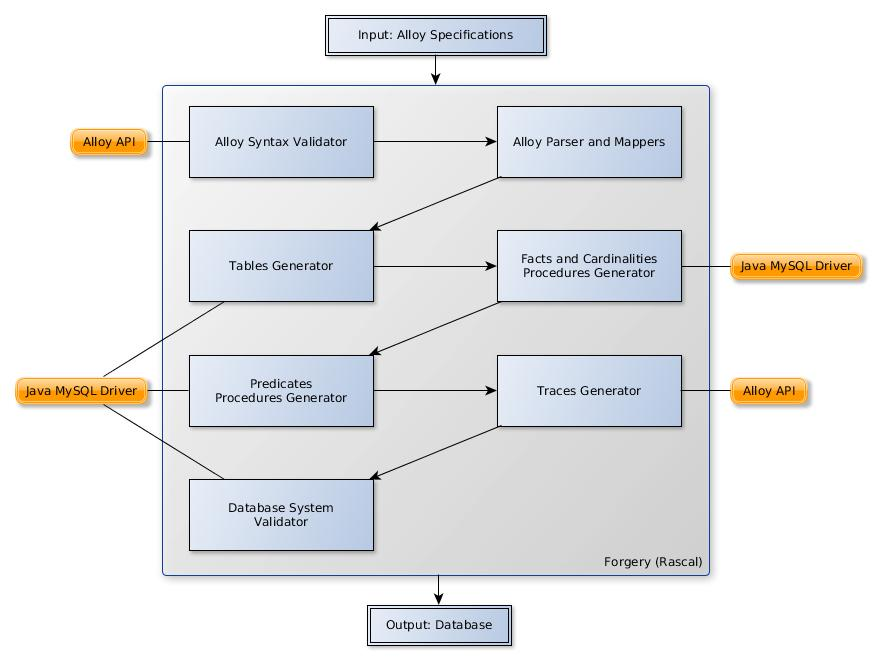
\includegraphics[scale=0.45]{forgery}
\caption{Forgery architecture}
\end{figure}

We implemented \textit{Forgery} using \textit{Rascal}. We chose \textit{Rascal} due to its powerful DSL and AST (Abstract Syntax Trees) tools. We used a standard SQL language. Therefore, any arbitrary database system can be used. We used \textit{MySQL} as it has large community. In this overview we will introduce the main points of how Forgery transform Alloy into SQL, and vital explanation for SQL.

\section{Alchemy Comparison}
Although related papers will be presented in a different chapter, there is a unique paper called Alchemy \cite{alchemy} that we 
have studied and due to overlapping research we will present it here. Similarly to Forgery, Alchemy compiles Alloy specifications into database implementation. We will discuss about the main differences here.\\

First, Alchemy generates a synthesizing API as a filtering layer that communicates with the database. In other words, the data validity can be guaranteed only when using this API. In contrast, Forgery generates a SQL system, the constraints are in the tables and the database level, hence it is more robust - the validity occurs on the data storing level. Also, SQL language is usually more familiar for technical people. And therefore, it may give a communication advantage.\\

Secondly, as introduced before, Alloy supports assertions for checking the model. Using the powerful Analyzer we able to detect mistakes in our specifications. Forgery supports assertions and even use their traces for evaluation. Alchemy introduced a shortcut to create predicates. However, those predicates specifications might be in contradiction to invariants. They added an auto-repair functionality that fix the data in case it is in conflict. However, the since the specifications are invalid by the nature of Alloy. The assertions and the analyzer cannot be used. Alchemy does not have evaluation method.\\

Thirdly, Alchemy does not generate command options to insert or delete atoms. By default, Forgery creates such procedures (With an option to create them manually).

\newpage

\section{Scheme Generation}
\label{sec:schemegen}

In this section we will discuss about how forgery generates the database scheme; including tables, fields etc. We will use the similar example as described in the overview with additional functionality and we will dive deeper into details.\\

\noindent The example describes a homework submission and grading system. Student's work may be submitted in pairs or individually. The gradebook stores the grade for each student on each submission. The system has some constraints and actions like enrolling students and so on, which we will not be discussed in this overview.\\
\begin{lstlisting}
sig Submission {}
sig Grade {}
sig Student {}
sig Course {
	roster: set Student,
	work: roster -> lone Submission,
	gradebook: work -> lone Grade
}
\end{lstlisting}

\noindent Alloy uses \textbf{sig}natures (e.g. Submission) to describe a data model \cite[p.~30]{alloy-manual}. Every signature defines the data type, and consists set of atoms drawn from that type. Atoms are elements that are created based on the system user's inputs. Forgery allows atoms to be created only within those signatures. \\

\noindent In addition, a signature can define fields (e.g. in Course). A field describes a relation between different types of Signatures. Basically, it is a set of tuples which consists different types of data. Such a relation can be unary or binary. E.g. roster and work respectively.

\newpage
\subsection{Atoms Tables}
\textbf{The signatures \textit{Student}, \textit{Submission}, \textit{Grade} and \textit{Course} are sets of atoms:}

\noindent$Student = \{Guy, Tijs, Jouke ..\}\\
Submission = \{homework, project ..\}\\
Grade = \{5.5, 8 ..\} \\
Course = \{Construction ..\}$\\

\noindent For each signature, atoms table is created. Every table has two fields: \textit{id} and \textit{value}.
The \textit{id} field is a primary key for identifying the atom, and \textit{value} is the input data.
Chosen types: \textit{Int} for \textit{id} as it is always an integer, and \textit{Varchar} for \textit{value} so it can contain any type of input (strings, numbers etc).

\begin{figure}[h!]
\centering
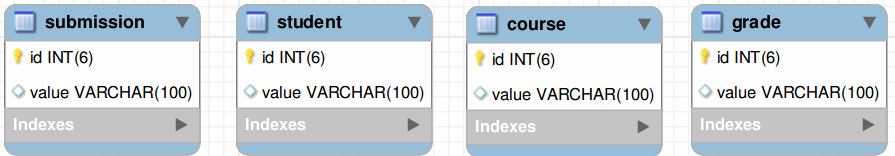
\includegraphics[scale=0.5]{1}
\caption{Generated tables for Signatures}
\end{figure}

\newpage
\subsection{Fields Relations}
\textbf{The signature \textit{Course} defines the following relations: roster (enrolled students), work and gradebook.}

\noindent$roster = \{<Construction, Guy>, <Construction, Tijs>..\}\\
work = \{<Construction, Guy, hwk1>.. \}\\
gradebook = \{<Construction, Guy, homework, 8> ..\}$\\

\noindent For every relation, a junction table is created. It describes the relationship between the different multiple relations and the atoms.
Every table contains the ids of the atoms that the relation describes. The table name is based on the relation name (right side before the colon sign $:$). Relation can be unary or binary. Binary relation is expressed by the tuple sign $\rightarrow$.\\

\noindent Moreover, Forgery adds SQL Foreign Keys that links between the tables. They are naturally extracted from the Alloy semantics. It guarantee that every junction table will contain valid data that points to existing atoms.\\

\noindent When a relation points to a another relation, Forgery extracts the atomic type. Which means, in other words, Forgery flattens all the relations so the tables will contain pointers to atomic tables only, and this way, the relationships between the tables would be simpler. It adds data redundancy but it makes the algorithm much more simpler.

\begin{figure}[h!]
\centering
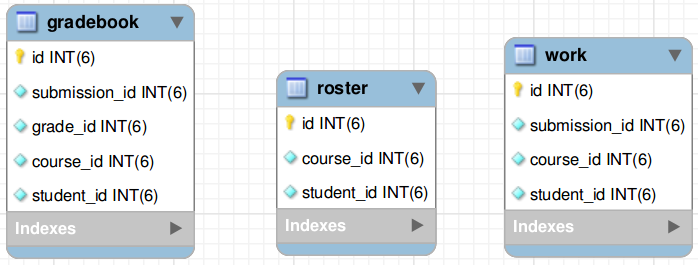
\includegraphics[scale=0.5]{2}
\caption{Generated tables for Relations}
\end{figure}

\newpage
\subsection{Cardinalities}
\noindent Alloy syntax supports multiple quantifiers to describe constraints on the data model: \textbf{\textit{lone}} (at most one atom), \textbf{\textit{some}} (at least one atom) and \textbf{\textit{one}} (single atom). Forgery uses two techniques to implement those constraints: \\

\noindent 1. Adding Unique Indexes for tables: the shared condition of \textit{lone}, \textit{one} and \textit{set} is that the table must not contain more than one similar element. Adding Unique Index guarantee this condition (although only partially/weaker condition for \textit{one}). \\

\noindent 2. Creating Stored Procedures: \textit{one} and \textit{some} cardinalities cannot be fully implemented by applying structural constraints into the SQL table itself. Therefore, we create a SQL procedure instead for each cardinality. The procedure contains a query that counts the rows and group it based on the cardinality criteria and then compare it to the specified cardinality. Those procedures are automatically called when the data is changed. If any violation occurs, the data will be reverted and error will be shown (transactional action). The cardinality procedures are stored in the database and can be identified with the prefix \textit{c\_}. More about procedures will be explained in the next chapter.
\newpage

\subsection{The Algorithm}
Let $S$ be a list of signatures, $s$ is a single signature, $R$ is its contained relations, $r$ is a single relation.\\

\begin{algorithm}
\caption{Database scheme mapper}
\label{array-sum0}
\begin{algorithmic}[1]
\Function{Create Scheme}{$S$}
	\State $tables = ()$ \Comment map (table name: list of fields)
	\For {each signature $s$ in $S$}
		\State \textbf{add} $(s.name: {id, value})$ \textbf{to} $tables$
		\For {each relation $r$ in $s.R$}
			\State $fields = \{\}$ \Comment set of table fields with cardinalities
			\State \textbf{add} $s.name$.`\_id` \textbf{to} fields
			\State \textbf{add} Atomic fields ($r.op1$, $tables$, $S$) \textbf{to} fields
			\If {$r.type$ is $Binary$}
				\State \textbf{add} Atomic fields ($r.op2$, $tables$, $S$) \textbf{to} fields
			\EndIf
			\State \textbf{add} $(r.name: fields)$ \textbf{to} $tables$
		\EndFor
	\EndFor
	\State \textbf{return} $tables$
\EndFunction
\end{algorithmic}
\end{algorithm}\newpage

\begin{algorithm}
\caption{Returns the most basic fields (Relations to their atoms)}
\label{array-sum1}
\begin{algorithmic}[1]
\Function{Atomic Fields}{$r,tables,S$}
			\If {$r.name$ in $S.names$}
				\State \textbf{return} $r.name$.`\_id`
			\EndIf
			\State \textbf{return} $tables[r.name]$
\EndFunction
\end{algorithmic}
\end{algorithm}

\begin{algorithm}
\caption{Returns the query}
\label{array-sum1}
\begin{algorithmic}[1]
\Function{Generate Query}{$tables$}
	\State $query = ""$
	\For {$table$ in $tables$}
		\State \textbf{add} SQL Statement ("Create Table", $table.name$) \textbf{to} $query$
		\For {$field$ in $tables[table]$}
			\State \textbf{add} SQL Statement ("Create Column", $field.name$) \textbf{to} $query$
			\State \textbf{add} SQL Statement ("Foreign Key", $field.name$) \textbf{to} $query$
			\If{$field.cardinality$ is $lone$ or $one$ or $set$} \State \textbf{add} SQL Statement ("Create Unique Index", $fields$) \textbf{to} $query$
			\EndIf
			\If{$field.cardinality$ is $some$ or $one$} \State \textbf{add} SQL Statement ("Create Cardinality Procedure", $fields$) \textbf{to} $query$
			\EndIf
		\EndFor
		\State \textbf{add} SQL Statement ("Create Column", $`id`$) \textbf{to} $query$
		\State \textbf{add} SQL Statement ("Create Primary Key", $`id`$) \textbf{to} $query$
	\EndFor
			\State \textbf{return} $query$
\EndFunction
\end{algorithmic}
\end{algorithm}

\newpage
\section{Predicates Generation}
\label{sec:predicatesgen}
This overview will discuss about the logic behind interpretation of Alloy predicates and creation of atoms. The same example from the previous chapter will be used with few additional statements.\\

\noindent The new statements introduces new features such as adding or deleting students, as they enroll in or drop the course, and assigning grades for each of their submitted work in pairs.\\

\begin{lstlisting}
sig Submission {}
sig Grade {}
sig Student {}
sig Course {
	roster: set Student,
	work: roster -> lone Submission,
	gradebook: work -> lone Grade
}
pred Enroll (c, c' : Course, _sNew : Student) {
	c'.roster = c.roster + _sNew and no c'.work [_sNew]
}
pred Drop (c, c' : Course, s: Student) {
	s not in c'.roster 
}
pred SubmitForPair (c, c' : Course, s1 : Student, s2 : Student, 
_bNew : Submission) {
	// pre-condition
	s1 in c.roster and
	s2 in c.roster and
	// update
	c'.work = c.work + (s1 -> _bNew) + (s2 -> _bNew)
}
pred AssignGrade (c, c' : Course, s : Student, b : Submission, 
g : Grade) {
	c'.gradebook = c.gradebook + (s -> b -> g)
}
\end{lstlisting}

\newpage
\subsection{Using Stored Procedures}

\noindent Stored Procedure is a SQL feature that encapsulates a query for re-usability purposes. It is used as a layer that communicates with the database internally. Stored Procedures allow faster execution time and they may be useful as a safer synthesizing mechanism (E.g. privileges) \cite{when}.\\

\noindent Basically, Stored Procedures are similar to other programming languages in that they can accept input parameters and return multiple values. Also, they may contain programming statements for performing operations in the database and indicate status of failure or success.\\

\noindent Forgery uses stored procedures for multiple purposes. One of them was already introduced in the previous overview in reference to cardinalities. Some others will be covered as well in this chapter.\\

\subsubsection{Alloy Predicates}

\noindent Alloy uses \textbf{pred}icates (e.g. Enroll) to capture the actions that are supported in the system. Each predicate describes the required state that the system should be in when applying it. Predicates has a header and a body. \\

\noindent\underline{Predicates Header:}

\noindent Predicates accept inputs from the user that are used for the states transformation. Each input contains a variable and a mapping to his belonged table. Similarly to Alchemy \cite{alchemy}, Forgery uses the prime symbol $'$ as a variable suffix to distinguish between pre- and post-states of the operation (e.g. $c$ and $c'$).\\

\noindent The inputs may be one of the two different types: an integer or a string. Inputs accept integers as default and each of them represents an Atom id. However, when it comes to a new Atom the id does not exist yet. Therefore, Forgery uses the underline symbol $\_$ in the variable prefix to refer to a new atom. In this case, the input type is a string, which is the data that the Atom carries. It may be a name of a course or a student and it may be just empty, depends on our model.\\

For each request for new atom, an Insert query will be added to the procedure, and the created id will be placed in the variable value. E.g. in our example $\_sNew : Student$ the generated query will be:
\begin{lstlisting}[escapechar=@,language=SQL]
INSERT INTO student(`value`) VALUES (_sNew);
SET _sNew = LAST_INSERT_ID();
\end{lstlisting}

\noindent\underline{Predicates Body:}

\noindent The predicates body may contain a formula in which the defined variables in the header are used.
The formula semantics of Alloy is based on the class of relational algebras. A predicate may define multiple formulas. Formulas are joined together using the $and$ word. Forgery handles them as a list of commands which performed serially one after one.\\

\noindent Forgery assumes that the formulas are correct by testing them in Alloy Checker\footnote{Not implemented yet.}. In addition, Forgery first checks whether the command refers to a pre- or post-condition and generates the query accordingly. For example, the Alloy membership test operator \textbf{in} will be converted into one of the following:\\

\noindent 1. Precondition is converted to "rollback if not exists" query (and the opposite for \textbf{not in}). Example: $s1$ in $c.roster$

\begin{lstlisting}[escapechar=@,language=SQL]
IF NOT EXISTS 
  (SELECT `id` FROM `roster` WHERE `student_id`=s1 AND `course_id`=c) 
THEN
  SELECT `An error has occurred, operation rollbacked 
  & the stored procedure was terminated`;
  ROLLBACK;
END IF;
\end{lstlisting}

\noindent 2. Postcondition is converted to "insert if not exists" query (and delete for \textbf{not in}): $s1$ in $c'.roster$

\begin{lstlisting}[escapechar=@,language=SQL]
IF NOT EXISTS 
  (SELECT `id` FROM `roster` WHERE `student_id`=s1 AND `course_id`=c) 
THEN
  INSERT INTO `roster` (`student_id`, `course_id`) VALUES(s1, c);
END IF;
\end{lstlisting}

\noindent\underline{More operators}:

\begin{enumerate}
\item Union - the operator $'+'$ is used to compute union of sets. Both sets must be of the same relation type and it is verified by Alloy Checker. Forgery makes the union using two different methods:

\begin{enumerate}
\item When the formula can be used equivalently with \textbf{in} operator (insert), similar method to \textbf{in} will be used (without existence testing). For example: $c'.roster = c.roster + s1$ is equivalent to $s1$ in $c'.roster$ (As all operations are transactional). Another example: $c'.roster = c.roster + s1 + s2$ is equivalent to $s1$ in $c'.roster$ and $s2$ in $c'.roster$.\\

\item In all other cases, the data in the table will be first flushed and then new data will be inserted\footnote{Not implemented yet.}.\\
\end{enumerate}

\noindent Alchemy uses framing conditions (e.g. $c'.gradebook = c.gradebook$). However, since Forgery execute all queries transactionally they are not needed (as mentioned before).\\

\item Difference - the operator $'-'$ works similarly to union, but with delete statements instead\footnote{Not implemented yet.}.\\

\item Join - operation is represented by square braces $[]$ (although in other languages it usually means array access). In our example the formula $no$ $c'.work [\_sNew]$ meant to verify that there is no work for this course that was submitted by the enrolling student. The generated query is:
\begin{lstlisting}[escapechar=@,language=SQL]
IF EXISTS
(SELECT id FROM `work` WHERE `student_id`=_sNew AND `course_id`=c)
 THEN
	SELECT `An error has occurred, operation rollbacked 
	and the stored procedure was terminated`;
	ROLLBACK;
END IF;
\end{lstlisting}

\item Tupling - represented by $\rightarrow$ symbol. Example: $c'.work = c.work + (s1 \rightarrow \_b) + (s2 \rightarrow \_b)$. The generated query is:
\begin{lstlisting}[escapechar=@,language=SQL]
INSERT INTO `work` (course_id, student_id, submission_id) 
	VALUES (c, s1, _bNew);
INSERT INTO `work` (course_id, student_id, submission_id) 
	VALUES (c, s2, _bNew);
\end{lstlisting}

\item Intersection - represented by $\&$ symbol. Supported only in facts (will not be discussed here).\\
\end{enumerate}

\subsubsection{Atoms Creation:}

\noindent Forgery supports two ways for creating new Atoms. The first way, which was introduced already is by using underline $\_$ variable prefix. The other way is by using the Forgery "create" procedures. Forgery automatically generates atom creation procedure for each signature. For example:
\begin{lstlisting}[escapechar=@,language=SQL]
DELIMITER //
CREATE PROCEDURE `create_submission`(IN atomVal VARCHAR(100))
BEGIN
DECLARE EXIT HANDLER FOR SQLEXCEPTION
BEGIN
	ROLLBACK;
END;

START TRANSACTION;
	INSERT INTO `submission` (`value`) VALUES (atomVal);
	-- facts and cardinalities are included here.
COMMIT;
END //
\end{lstlisting}

\noindent As mentioned before, \textit{Forgery} verifies all the invariants (cardinalities and facts) in each procedure. This rule applies here. This means that if there is any violation, the data will be reverted.

\newpage

\begin{figure}[h!]
\centering
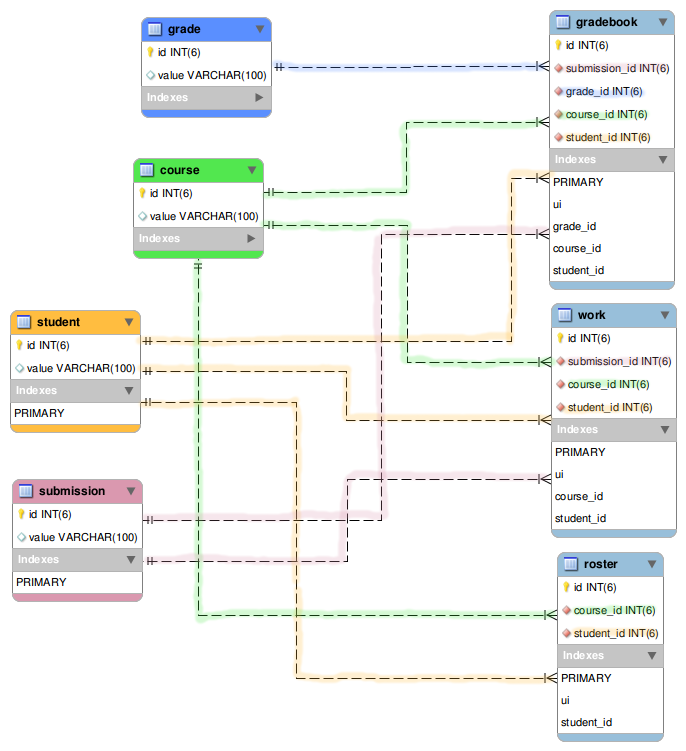
\includegraphics[scale=0.5]{3}
\caption{Generated Relational Database}
\end{figure}

\newpage

\section{Validation}
\label{sec:validation}

\subsection{Reverse Engineering}
While \textit{Alloy} search for models, it generates traces and saves them as a temporary XML file. Those traces are the operations that were performed in the system and they create the possible models or counter examples.

The idea was to use those traces for duplicating the operations in \textit{Forgery's} database and then comparing the results to those in \textit{Alloy} for tests purposes. In other words, applying reverse engineering on the results of \textit{Alloy}. However, the traces miss some important information.\\ 

By default, the traces are not ordered and this has to be configured manually. Otherwise, they are useless because we cannot know the data flow. To order them, the ordering library has to be included and initialized using $init$ predicate (ignored in Forgery). And also, the logic behind the steps progress from one to another has to be defined using $traces$ fact (also ignored in Forgery).\\ 

Besides, the operation name that leaded to a new state is not saved so we able to know only the data of the new state (Atoms and the Relations) but not who caused i. Therefore, to deal with it we made a small trick. We added an arbitrary atom called $operation_id$ and his value is connected to each operation and identifies it uniquely. For example:\\

\begin{lstlisting}
open util/ordering[Course] as CourseOrder
sig Student {}
sig Course {
	roster : set Student,
	operation_id: Int
}

pred Enroll (c, c' : Course, _st : Student) {
	c'.roster = c.roster + _st
	and c'.operation_id = 1 
}

pred init(c: Course) {
	no c.roster
	and c.operation_id = 0
}

fact traces{
    init[first]
    all c: Course - last | let c' = next[c] | 
	some st: Student |
	Enroll[c,c',st]
}
\end{lstlisting}

\textit{Alloy's} output:\\
\begin{center}
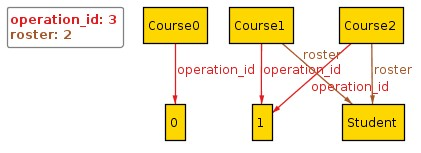
\includegraphics[scale=0.7]{output_traces}
\end{center}

The data flow:
\begin{enumerate}
	\item Initializing (0): The precondition for the initializing state is that there are no students enrolled and therefore no students enrolled to Course0.
	\item Enrolling (1): The student is enrolled to Course1.
	\item Enrolling (1): The student is enrolled to Course2.
\end{enumerate}

\subsection{Validation Scenarios}

In order to validate \textit{Forgery's} output we have to consider the following scenarios:
\begin{center}
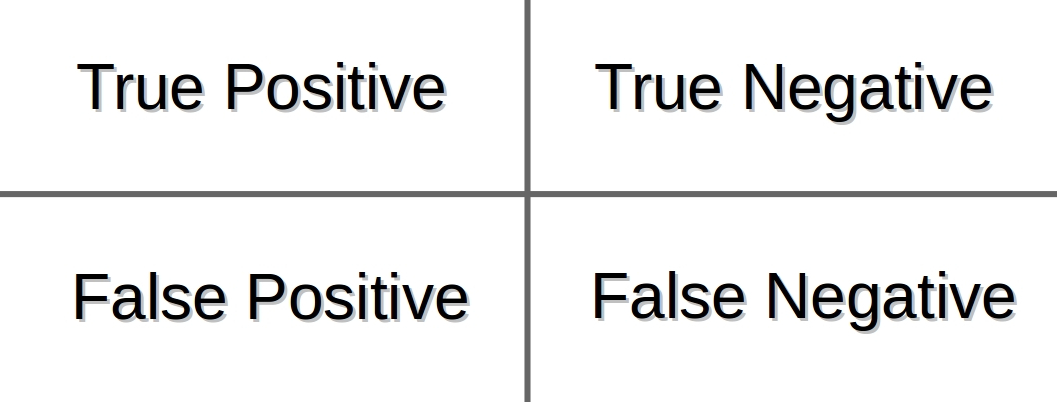
\includegraphics[scale=0.25]{scenarios}
\end{center}

\begin{comment}
\begin{enumerate}
  \item True Positive: Correct models in \textit{Alloy} and in \textit{Forgery}.
  \item False Positive: Incorrect models in \textit{Alloy} but correct in \textit{Forgery}.
  \item True Negative: Incorrect models in \textit{Alloy} and in \textit{Forgery}.
  \item False Negative: Correct models in \textit{Alloy} but incorrect in \textit{Forgery}.
\end{enumerate}
\end{comment}

\subsubsection{True Positive - False Negative}
\begin{itemize}
  \item True Positive: Correct models in \textit{Alloy} and in \textit{Forgery}.
  \item False Negative: Correct models in \textit{Alloy} but incorrect in \textit{Forgery}.
\end{itemize}

We have to irritate over all the correct \textit{Alloy} models and test them in \textit{Forgery} using the traces as described before.

\subsubsection{True Negative - False Positive}
\begin{itemize}
  \item True Negative: Incorrect models in \textit{Alloy} and in \textit{Forgery}.
  \item False Positive: Incorrect models in \textit{Alloy} but correct in \textit{Forgery}.
\end{itemize}

\textit{Alloy} supports policy constraints. One of them which has been already introduced is a $fact$. Another type but similar is $assert$. While a fact is used to force something to be true of the model, an assert is a claim that something must already be true due to the rest of the model \cite{alloytutorial}. Assertions are used mostly to test the predicates. They verify that the specified model is correct and that we used the desirable conditions (e.g. not too weak).\\

Similarly to finding models, Alloy uses the Assertions to find counterexamples for the model. Traces are also generated in this case, and we able to use them to test \textit{Forgery} too.

\newpage

\chapter{Related Work}

Alloy is increasingly becoming popular declarative modelling language thanks to providing early error detection, supported by automated model analysis tools for simulating and debugging models \cite{lightning}. Therefore, there were few related papers that were written.

\section{From UML to Alloy and Back Again}
This paper presents a study involving UML2Alloy, a tool for transforming
UML models in form of UML class diagrams which are augmented with
OCL constraints, to Alloy. The conversion allows analysis of UML models
via Alloy, to identify consistencies in those UML models.

\section{Alchemy: Transmuting Base Alloy Specifications into Implementations}
We present Alchemy, which compiles Alloy specifications into implementations that execute against persistent databases. Alchemy translates a subset of Alloy predicates into imperative update operations, and it converts facts into database integrity constraints that it maintains automatically in the face of these imperative actions.

\section{Mapping between Alloy specifications and database implementations}
An abstract Alloy specification is far from an actual implementation, and manually refining the former into the latter is unfortunately a non-trivial task. This paper identifies a subset of the Alloy language that is equivalent to a relational database schema with the most conventional integrity constraints, namely functional and inclusion dependencies.

\section{Towards an Operational Semantics for Alloy}
In this paper we demonstrate the subtlety of representing state in Alloy speci- fications. We formalize a natural notion of transition semantics for state-based specifications and show examples of specifications in this class for which analy- sis based on relational algebra can induce false confidence in designs.

\newpage

\chapter{Conclusions}

In this work we presented \textit{Forgery} as a tool that supports the realization of \textit{Alloy} based specifications. We able to generate a full-scale database including structural tables, constraints and functions for data updating operations. The output is a pure SQL that doesn't require any external API or additional dependencies. In addition, it is easily expandable by using different SQL features. For example it is possible to manage privileges of users and that way increasing security.\\ 

As mentioned before, it is not possible to develop fault-free software in practical scenario considering human nature \cite{reliability}. That also applies for \textit{Forgery}. Hence, we developed a validation mechanism with reverse engineering that allows to compare the results to those in \textit{Alloy}. Moreover, enabling Assertions helps to find issues in the model; A feature that was not possible in Alchemy.\\

Together with \textit{Fors} we created a toolchain that supports the main software development processes: modelling and implementation. Those two important processes have direct affect on the software quality. By improving them organizations might save lot of money and other resources.\\

There are still challenges to be solved in \textit{Forgery},for instance, expanding the set of supported \textit{Alloy} syntax and resolving potential exceptions. However, to the best of our knowledge, considering multiple scenarios, \textit{Forgery} has achieved his goals. 

\begin{thebibliography}{9}

\bibitem{requirements}
  Pete Sawyer and Gerald Kotonya, 
  \emph{Software Requirements} (IEEE, 2001).
  
\bibitem{dsl}
  Walid Taha, 
  \emph{Domain-Specific Languages} (Rice University, 2008).
  
\bibitem{fors}
  Chiel Peters, 
  \emph{Fors: Separating Configuration From Formal Specification} (University of Amsterdam, 2014).
  
\bibitem{alchemy}
  Daniel J. Dougherty et al, 
  \emph{Alchemy: Transmuting Base Alloy Specifications
into Implementations} (Worcester, 2008).

\bibitem{abstractions}
  Daniel Jackson, 
  \emph{Software Abstractions: Logic, Language and Analysis} (MIT, 2012).
  
\bibitem{security}
  Sabrina De Capitani et al, 
  \emph{Database Security} (Wiley, 2002).
  
\bibitem{lightning}
  Loic Gammaitoni et al, 
  \emph{Verifying Modelling Languages using Lightning} (University of Luxembourg, 2014).

\bibitem{reliability}
  Ajeet Kumar et al, 
  \emph{Early Software Reliability Prediction: A Fuzzy Logic Approach} (Springer, 2013).
  
\bibitem{alloytutorial}
  Rob Seater and Greg Dennis, 
  \emph{Tutorial for Alloy Analyzer 4.0} (MIT, 2014).
  
\bibitem{defectstopten}
  Barry Boehm and Victor R. Basili, 
  \emph{Software Defect Reduction Top 10 List} (IEEE, 2001).
  
\bibitem{when}
  Tony Patton, 
  \emph{Determine when to use stored procedures vs. SQL in the code} (TechRepublic, 2005).  
  
\bibitem{sqlalgebra}
  T. M. Murali, 
  \emph{SQL and Relational Algebra} (VirginiaTech Engineering College, 2010).   
  
\bibitem{minimizingdefects}
  Khaleel Ahmad and Nitasha Varshney, 
  \emph{On Minimizing Software Defects during New Product Development Using Enhanced Preventive Approach} (IJSCE, 2012).

\bibitem{alloy-manual}
  Daniel Jackson, 
  \emph{Micromodels of software: lightweight modelling and analysis with Alloy} (MIT, 2002).

\bibitem{datastruct}
  Michael Brackett, 
  \emph{Data Architecture and Data Structures} (DATAVERSITY, 2013).  
 
\bibitem{introtodb}
  Christopher J. Date, 
  \emph{An Introduction to Database Systems} (Pearson, 2003).  


\end{thebibliography}

\chapter{Appendix}
\section{Alloy Quick Reference}

Full Reference: http://www.ics.uci.edu/~alspaugh/cls/shr/alloy.html

\subsection{Logic}
The Alloy logic is a first-order logic in which the domain is the set of all relations, and terms include relational expressions such as joins.~

Everything in Alloy is a relation!~

\begin{itemize}
\item A relation is a set of tuples of the same (positive) arity.~ Each tuple lists entities that are related to each other.~ The size of the relation is the number of tuples; the arity of the relation is the arity of the tuples.~
\item Sets are represented by unary relations.~ Each 1-tuple in the unary relation contains an element of the set.~
\item Scalars are represented by~singleton sets.~ Since a set is a unary relation, an scalar is thus represented as a singleton (size 1) unary relation.~
\end{itemize}
As a result, the operators apply to relations, sets, and scalars, and there are very few cases that produce no result.~

Page numbers refer to Daniel Jackson,~Software Abstractions, MIT Press 2006.~

\newpage

\subsection{Syntax}
\begin{flushleft}
\tablefirsthead{}
\tablehead{}
\tabletail{}
\tablelasttail{}
\begin{supertabular}{|m{0.33235985in}|m{1.1580598in}|}
\hline
\multicolumn{2}{|m{1.5691599in}|}{\centering Set constants~50}\\\hline
univ &
The universal set\\\hline
none &
The~empty set\\\hline
\end{supertabular}
\end{flushleft}
\begin{flushleft}
\tablefirsthead{}
\tablehead{}
\tabletail{}
\tablelasttail{}
\begin{supertabular}{|m{0.33235985in}m{1.3830599in}|}
\hline
\multicolumn{2}{|m{1.7941599in}|}{\centering Relation constants~50}\\\hline
\multicolumn{1}{|m{0.33235985in}|}{iden} &
The~identity relation\\\hline
\end{supertabular}
\end{flushleft}
\begin{flushleft}
\tablefirsthead{}
\tablehead{}
\tabletail{}
\tablelasttail{}
\begin{supertabular}{|m{0.5400598in}|m{0.78025985in}|m{0.47685984in}|}
\hline
\multicolumn{3}{|m{1.9546599in}|}{\centering Set operators~52}\\\hline
\centering Symbol &
\centering Name &
\centering\arraybslash Result\\\hline
+ &
Union &
A set\\\hline
\& &
Intersection &
\\\hhline{--~}
{}- &
Difference &
\\\hline
in &
Subset &
T or F\\\hline
= &
Equality &
\\\hhline{--~}
\end{supertabular}
\end{flushleft}

\begin{flushleft}
\tablefirsthead{}
\tablehead{}
\tabletail{}
\tablelasttail{}
\begin{supertabular}{|m{0.5400598in}|m{1.94416in}|m{0.6073598in}|}
\hline
\multicolumn{3}{|m{3.24906in}|}{\centering Relation operators~55}\\\hline
\centering Symbol &
\centering Name &
\centering\arraybslash Syntax\\\hline
{}-{\textgreater} &
(Arrow)~product &
R1~-{\textgreater}~R2\\\hline
. &
Join &
R1~.~R2\\\hline
[] &
Join (a second notation for it) &
R2~[R1]\\\hline
\~{} &
Transpose &
\~{}~R\\\hline
\^{} &
Transitive closure &
\^{}~R\\\hline
* &
Reflexive transitive closure &
*~R\\\hline
{\textless}: &
Domain restriction &
Set~{\textless}:~R\\\hline
:{\textgreater} &
Range restriction &
R :{\textgreater}~Set\\\hline
++ &
Override &
R1~++~R2\\\hline
\end{supertabular}
\end{flushleft}
\begin{flushleft}
\tablefirsthead{}
\tablehead{}
\tabletail{}
\tablelasttail{}
\begin{supertabular}{|m{0.5400598in}|m{0.6525598in}|m{2.2740598in}|}
\hline
\multicolumn{3}{|m{3.6241598in}|}{\centering Logical operators~69}\\\hline
\centering Symbol &
\centering Keyword &
\centering\arraybslash Name or result\\\hline
! &
not &
negation\\\hline
\&\& &
and &
conjunction\\\hline
{\textbar}{\textbar} &
or &
disjunction\\\hline
={\textgreater} &
implies &
implication\\\hline
{\textless}={\textgreater} &
iff &
logical equivalence\\\hline
~
 &
else &
A={\textgreater}B~else~C~${\equiv}$~(A\&\&B){\textbar}{\textbar}(!A\&\&C)\\\hline
\end{supertabular}
\end{flushleft}

\begin{flushleft}
\tablefirsthead{}
\tablehead{}
\tabletail{}
\tablelasttail{}
\begin{supertabular}{|m{0.33235985in}|m{1.5545598in}|m{1.5712599in}|}
\hline
\multicolumn{3}{|m{3.6156597in}|}{\centering Quantifiers/predicates~70}\\\hline
~
 &
\centering Quantification\newline
Q var:set {\textbar} formula &
\centering\arraybslash Predicate on relations\newline
Q e\\\hline
all &
universal &
—\\\hline
some &
existential &
size is 1 or greater\\\hline
no &
¬${\exists}$ &
size is 0\\\hline
lone &
zero or one exists &
size is 0 or 1\\\hline
one &
exactly one exists &
singleton\\\hline
\end{supertabular}
\end{flushleft}

\begin{flushleft}
\tablefirsthead{}
\tablehead{}
\tabletail{}
\tablelasttail{}
\begin{supertabular}{|m{0.81365985in}m{3.6025598in}|}
\hline
\multicolumn{2}{|m{4.49496in}|}{\centering let~73}\\\hline
\multicolumn{1}{|m{0.81365985in}|}{let~x~=~e~{\textbar}~A} &
A~with every occurrence of~x~replaced by expression~e\\\hline
\end{supertabular}
\end{flushleft}
\subsubsection{Signatures and relations}
(Parts of this subsection describe the~Alloy language.)

Each set of atoms is defined by a~signature, with keyword~sig.~

A signature can contain zero or more relation~declarations, separated by commas. Each declaration names a (binary) relation between the set defined by the signature and a set or relation.

\begin{verbatim}
  //  Simple example
  abstract sig Person {     // Signature
    father: lone Man,       //   A declaration
    mother: lone Woman      //   Another declaration
  }
  sig Man extends Person {
    wife: lone Woman
  }
  sig Woman extends Person {
    husband: lone Man
  }
\end{verbatim}
\begin{flushleft}
\tablefirsthead{}
\tablehead{}
\tabletail{}
\tablelasttail{}
\begin{supertabular}{|m{0.8580598in}|m{0.6323598in}|m{0.97815984in}|m{1.5976598in}|}
\hline
\multicolumn{4}{|m{4.3024597in}|}{\centering Relationships among signatures}\\\hline
S~in~T~\newline
U~in~T &
subset &
Every~S~is a~T,~\newline
and~\newline
every~U~is a~T &
An~S~can also be a~U\\\hline
S~extends~T~\newline
U~extends~T &
extension &
 &
An~S~cannot also be a~U\\\hhline{--~-}
\end{supertabular}
\end{flushleft}
The extended signature must be either a top-level signature or a subsignature.~

\subsubsection{Constraining a declaration}
There are two ways:~

\begin{enumerate}
\item with~set~or~relation~multiplicity constraints in the signature.~ These are a quick shorthand.~ The~example above~has several of these (all are~lone).
\item with a~fact~117~that states a constraint on the set or relation.~ The constraint is expressed in the Alloy logic.~

(The~fact~keyword may be omitted if the fact is only about the relations of a single signature, and it immediately follows that signature — then it is a~signature fact, and is implicitly universally quantified over the signature's set, and may use~this~as if it were the variable of this implied quantification.)~
\end{enumerate}

\subsubsection{Multiplicity constraints in declarations}

\bigskip

\begin{flushleft}
\tablefirsthead{}
\tablehead{}
\tabletail{}
\tablelasttail{}
\begin{supertabular}{|m{0.60315984in}|m{2.24766in}|}
\hline
\multicolumn{2}{|m{2.92956in}|}{\centering Set declarations with multiplicities~76}\\\hline
\multicolumn{2}{|m{2.92956in}|}{\centering e~is a expression producing a set (arity 1)}\\\hline
x:~set~e &
x~a subset of~e\\\hline
x:~lone~e &
x~empty or a singleton subset of~e\\\hline
x:~some~e &
x~a nonempty subset of~e\\\hline
x:~one~e &
x~a singleton subset of~e\newline
(i.e. a scalar)\\\hline
x:~e &
x~a singleton subset of~e\newline
(equivalent to~one)\\\hline
\end{supertabular}
\end{flushleft}

\bigskip

\begin{flushleft}
\tablefirsthead{}
\tablehead{}
\tabletail{}
\tablelasttail{}
\begin{supertabular}{|m{1.1573598in}m{3.79346in}|}
\hline
\multicolumn{2}{|m{5.02956in}|}{\centering Relation declarations with~-{\textgreater}~multiplicities~77}\\\hline
\multicolumn{2}{|m{5.02956in}|}{\centering A~and~B~are expressions producing a relation~\newline
m~and~n~are~some,~lone,~one, or not present (which is equivalent to~set)}\\\hline
\multicolumn{1}{|m{1.1573598in}|}{r:~A~m~-{\textgreater}~n~B} &
m~elements of~A~map to each element of~B\\\hline
 &
each element of~A~maps to~n~elements of~B\\\hhline{~-}
\end{supertabular}
\end{flushleft}
\subsubsection{Facts}
117~A~fact~contains a formula in the Alloy logic that is assumed to always be true. See the~Alloy language~for more details.~

\subsubsection{Disjointness}
71~disj~before a list of variables restricts their bindings to be disjoint.~

\subsubsection{Cardinality constraints}
80~The prefix operator~\#~(cardinality) on a relation produces the relation's size.~ The result can be operated on with~+ - = {\textless} {\textgreater} ={\textless} {\textgreater}=.~ Positive integer literals can appear in cardinality expressions.~

sum~x:~e~{\textbar}~ie~sums the value of~ie~for each~x~in set~e.~

\subsection{Modelling}
The Alloy language uses the Alloy logic plus some other constructs to make~models.~ In Alloy, a model is {\textquotedbl}a description of a software abstraction{\textquotedbl}~4.~

(Recall that in FOL a model means~something different.)~

\subsubsection{Language constructs}
The Alloy language adds these constructs to the~Alloy logic:~

\begin{enumerate}
\item A~module~line gives the relative pathname of the model's file (minus the {\textquotedbl}.als{\textquotedbl} suffix).~ The pathname is relative to the directory that imported module pathnames are going to be relative to.~ (Obviously, the~module~line is mostly redundant with the file's full pathname.)~
\item A~sig~(signature) declares one or more sets of atoms, and their relations to other sets.~
\item A~fun~(function) defines a way of getting a relation (or set, or atom).~ It can take parameters that are used in getting its result.~ It can define a relation (usually using~-{\textgreater}) and make use of it to produce its result.~ It is a~FOL function~for the Alloy logic, in which expressions are relations.~
\item A~pred~(predicate) defines a formula (true or false).~ It can take parameters that are used in getting its result.~ It is a~FOL predicate~for the Alloy logic.~
\item A~fact~defines a formula that you assume is valid (always true, for any world).~ The Alloy analyzer uses~facts as axioms in constructing its examples and counterexamples.~
\item You~run~a~predicate in order to see the examples (if any) the Alloy analyzer finds for which the predicate is true.~

You define the~scope~that the analyzer checks by saying things like {\textquotedbl}run for 3{\textquotedbl} or {\textquotedbl}run for 3 but 4 Dog{\textquotedbl}.~ The analyzer will then check only possible examples that contain no more than that many of atoms from each set.~

If it finds an example, then the predicate is~satisfiable.~

If it finds no examples, the predicate may be either~invalid~(false for all possible examples); or it may be~satisfiable~but not within the scope you used.~
\item An~assert~(assertion) defines a formula that you claim will always be true.~ An~assertion differs from a~fact~in that the Alloy analyzer will check an~assertion to see if it is true for all the examples in a scope, whereas the analyzer assumes each~fact~is true and uses them to constrain which examples it looks at.~
\item You~check~an~assertion in order to see whether the Alloy analyzer finds any counterexamples.~

You define the scope as for a~run~command.~

If it finds a counterexample, then the predicate is~unsatisfiable.~

If it finds no counterexamples, the predicate may be either~valid~(true for all possible examples); or it may be~unsatisfiable~but not within the scope you used.~
\end{enumerate}
\subsubsection{Which construct to use where?}
\begin{enumerate}
\item Writing a model (Alloy file) that might need to import other models?~ Use~module.~
\item Need a set of atoms?~ Use a~sig.~
\item Need an expression, whose value is a function (or set, or scalar)?~ Use a~fun~(function).~
\item Need a formula, whose value is true or false?~ Use a~pred~(predicate).~
\item Need to state an axiom that you want to be true always?~ Use a~fact~(function).~
\item Need an example for which a~pred~is true?~~run~the predicate to see if one exists.~ It's like using an existential quantifier over all the predicate's parameters.~
\item Want to claim something is always true?~ Use an~assert~(assertion).~
\item Want to see if an~assert~is unsatisfiable?~~check~the assertion to see if any counterexample can be found.~
\end{enumerate}
\subsection{Signatures}

\bigskip

\begin{flushleft}
\tablefirsthead{}
\tablehead{}
\tabletail{}
\tablelasttail{}
\begin{supertabular}{|m{1.6816599in}|m{3.68236in}|}
\hline
\multicolumn{2}{|m{5.44276in}|}{\centering Signatures~91}\\\hline
sig~A~\{fields\} &
Declares a set~A~of atoms\\\hline
sig~A~extends~B~\{fields\} &
Declares a subset~A~of set~B, disjoint from~\newline
all other~extends~subsets of~B\\\hline
sig~A~in~B~\{fields\} &
Declares a subset~A~of~B\\\hline
sig~A~in~B~+~C~\{fields\} &
Declares a subset~A~of the union (+) of sets~B~and~C\\\hline
abstract sig~A~\{fields\} &
Declares a set~A~that contains no atoms\newline
other than the ones in its subsets (if any)\\\hline
one~ sig~A~\{fields\} &
Declares a singleton set~A\\\hline
lone sig~A~\{fields\} &
Declares a set~A~of 0 or 1 atom\\\hline
some sig~A~\{fields\} &
Declares a nonempty set~A\\\hline
sig~A,~B~\{fields\} &
Declares two sets~A~and~B~of atoms\newline
Wherever~A~appeared above, a list of names can appear\\\hline
\end{supertabular}
\end{flushleft}

\bigskip

\begin{flushleft}
\tablefirsthead{}
\tablehead{}
\tabletail{}
\tablelasttail{}
\begin{supertabular}{|m{1.7309599in}|m{3.0802598in}|}
\hline
\multicolumn{2}{|m{4.88996in}|}{\centering Fields (in a signature for set~A)~95}\\\hline
f:~e &
Declares a relation~f~that's a subset of~A-{\textgreater}e.~\newline
e~can be any expression that produces a set —\newline
union, intersection, ... , any combination.\\\hline
f: lone~e &
Each~A~is related to no~e~or one~e.\\\hline
f: one~e &
Each~A~is related to exactly one~e.\\\hline
f: some~e &
Each~A~is related to at least one~e.\\\hline
f:~g-{\textgreater}h &
Each~A~is related to a relation from~g~to~h.\\\hline
f: one~g~lone -{\textgreater} some~h &
The multiplicities have their~usual meanings.\newline
Here, each~A~is related to exactly one relation\newline
relating each~g~to 1 or more~h's, and\newline
each~h~is related to 0 or 1~g.\\\hline
\end{supertabular}
\end{flushleft}
\subsection{Functions}
\begin{flushleft}
\tablefirsthead{}
\tablehead{}
\tabletail{}
\tablelasttail{}
\begin{supertabular}{|m{2.11566in}m{4.41986in}|}
\hline
\multicolumn{2}{|m{6.6142597in}|}{\centering Function~121s}\\\hline
\multicolumn{1}{|m{2.11566in}|}{fun~Name~[parameters] :~type~\{e\}} &
Defines a function, with the given~name~and (possibly empty)~parameters,\newline
and producing a relation (or set, or scalar) of the given~type.~\newline
The result is defined by the expression~e, which may reference the~parameters.~\\\hline
\end{supertabular}
\end{flushleft}
\subsection{Predicates}
\begin{flushleft}
\tablefirsthead{}
\tablehead{}
\tabletail{}
\tablelasttail{}
\begin{supertabular}{|m{1.8295599in}m{4.70596in}|}
\hline
\multicolumn{2}{|m{6.6142597in}|}{\centering Predicates~121}\\\hline
\multicolumn{1}{|m{1.8295599in}|}{pred~Name~[parameters]~\{f\}} &
Defines a predicate, with the given~name~and (possibly empty)~parameters.~\newline
A predicate always produces true or false, so no type is needed.~\newline
The result is defined by the formula~f, which may reference the~parameters.~\\\hline
\end{supertabular}
\end{flushleft}
\subsection{Facts}
\begin{flushleft}
\tablefirsthead{}
\tablehead{}
\tabletail{}
\tablelasttail{}
\begin{supertabular}{|m{1.0219599in}|m{2.69346in}|}
\hline
\multicolumn{2}{|m{3.79416in}|}{\centering Facts~117}\\\hline
fact \{e\} &
The expression~e~is a constraint that~\newline
the analyzer will assume is always true.~\\\hline
fact~Name~\{e\} &
You can name a~fact~if you wish;\newline
the analyzer will ignore the name.\\\hline
\end{supertabular}
\end{flushleft}
\subsection{Assertions}
\begin{flushleft}
\tablefirsthead{}
\tablehead{}
\tabletail{}
\tablelasttail{}
\begin{supertabular}{|m{1.1538599in}m{4.91566in}|}
\hline
\multicolumn{2}{|m{6.14826in}|}{\centering Assertions~124}\\\hline
\multicolumn{1}{|m{1.1538599in}|}{assert~Name~\{f\}} &
Defines a assertion, with the given~name.~ Assertions take no parameters.~\newline
An assertion always produces true or false, so no type is needed.~\newline
The result is defined by the formula~f.~\\\hline
\end{supertabular}
\end{flushleft}

\bigskip


\end{document}